\chapter{$\mathcal{N} = 4$ SYM}

Consider the action of a $d$-dimensional Yang-Mills (YM) theory 
with a massless spin-$\frac{1}{2}$ field $\Psi$ in the adjoint representation of the gauge group $U(N)$:
% (we will consider $SU(N)$)
\begin{equation}
 S = - \dfrac{1}{g_{YM}^2} \int d^d x \, \text{tr}
     \left(
         \dfrac{1}{2}F_{M N}F^{M N}
       - \bar{\Psi} \Gamma^M D_M \Psi 
     \right),    
\end{equation}
where $F_{M N} =\sum_{a=1}^{N^2} F_{M N}^a T^a_{ij}$, so that the trace is over the matrix indices $i, j=1, \ldots, N$. 
$T^a$ are the generators of the gauge group.
More explicitly, the field-strength and the covariant derivative are
\begin{eqnarray}
 F_{MN} &=& \partial_M A_N - \partial_N A_M + [A_M, A_N],\\
 D_M &=& \partial_M  + [A_M, \cdot].
\end{eqnarray}

% \begin{eqnarray}
%  F_{MN}^a &=& \partial_M A_N^a - \partial_N A_M^a + f_{abc} A_M^b A_N^c,\\
%  D_M \Psi^a &=& \partial_M \Psi^a + f_{abc} A_M^b \Psi^c,
% \end{eqnarray}
% where the structure constants $f_{abc}$ are defined by the commutation relation $[T^a, T^b]=f_{abc} T^c$.


In Minkowski spacetime $\mathbb{R}^{9,1}$, 
this action turns out to be invariant under the supersymmetry transformation:
\begin{eqnarray}
 \delta_\epsilon A_M  & = & \epsilon \Gamma_M \Psi,\\
 \delta_\epsilon \Psi & = & \dfrac{1}{2} F_{M N} \Gamma^{M N} \epsilon,
\end{eqnarray}
where $\epsilon$ is a constant Majorana-Weyl spinor that parametrizes the transformation.
% The bosonic and the fermionic degrees of freedom indeed match,
% \begin{itemize}
%  \item Bosonic: $D-2 = 8$
%  \item Fermionic: $2^{D/2}/2/2 = 8$
% \end{itemize}
% which is a necessary condition for supersymmetry. 

 
Lower dimensional supersymmetric theories can actually be obtained by 
dimensional reduction from the above theory \cite{Brink:1976bc}. 
Let us review how we can derive the action for the maximally supersymmetric
$\mathcal{N}=4$ SYM on $\mathbb{R}^{4}$.

\section{Action on $\mathbb{R}^{4}$}
The dimensional reduction consists of restricting the dependence of the fields only to 4 dimensions: $(x_1, \ldots, x_4)$.
The original Lorentz symmetry group $Spin(9,1)$ is then broken to $Spin(4) \times Spin(5,1)^R$,
that is the Lorentz group in 4d and an internal symmetry group called R-symmetry (hence the superindex $R$).
These groups are isomorphic to:
\begin{eqnarray}
Spin(4)      &=& SU(2)_L \times SU(2)_R \\
Spin(5, 1)^R &=& Spin(4)^R \times SO(1,1)^R \\
	     &=& SU(2)^R_L \times SU(2)^R_R \times SO(1,1)^R.
\end{eqnarray}
% where the subindexes $L, R$ refers to left and right. 

The gauge field $A_M$ is reduced to the 4d gauge field and scalars:
\begin{eqnarray}
 Spin(4):     & \,& A_\mu, \quad \mu = 1, 2, 3, 4 \\
%  Spin(5,1)^R: & \,& \Phi_I, \quad I = 0, 5, 6, 7, 8, 9
 Spin(4)^R: & \,& \Phi_I, \quad I = 5, 6, 7, 8 \\
 SO(1,1)^R: & \,& \Phi_I, \quad I = 0, 9 
\end{eqnarray}
where we wrote down the group they transform under.

The fermionic field, which is a Majorana-Weyl spinor, 
can be decomposed to 4 Majorana spinors (each having 2 degrees of freedom):
\begin{equation}
 \Psi=\begin{bmatrix}
       \psi_L\\
       \chi_R\\
       \psi_R\\
       \chi_L
      \end{bmatrix}
\end{equation}
where the spinors with the subindex $L$ (or $R$) transform in the spin-$\frac{1}{2}$ representation of
$SU(2)_L$ (or $SU(2)_R$).
Also, spinors with the name $\psi$ and $\chi$ transform in the spin-$\frac{1}{2}$ representation of
$SU(2)_L^R$ and $SU(2)_R^R$ from the R-symmetry subgroup, respectively.




The $\mathcal{N}=4$ SYM action explicitly written in terms of the 4d bosonic fields is:
\begin{equation}\label{SR4}
  \begin{split}
    S_{\mathbb{R}^4} = - \dfrac{1}{g_{YM}^2} \int d^4 x \, \text{tr}
    (
         \dfrac{1}{2}F_{\mu \nu}F^{\mu \nu}
       + D_\mu \Phi_I D^\mu \Phi^I
       + \dfrac{1}{2} [\Phi_I, \Phi_J]\, [\Phi^I, \Phi^J]       
    \\
       \qquad
       - \bar{\Psi} \Gamma^\mu D_\mu \Psi 
       - \bar{\Psi} \Gamma^I [ \Phi_I, \Psi ]
    ),
   \end{split}
\end{equation}
where we decomposed the 10d gamma matrices as $\Gamma^M=\Gamma^\mu \otimes \Gamma^I$.


The action has no mass scale, and it is in fact conformal invariant even at quantum level \cite{MANDELSTAM1983149, BRINK1983323}.
The conformal group extends the Poincar\'e group (translation, rotations and boosts) 
to include scaling (dilatation),
and special conformal transformation, which is a composition of inversion, translation and inversion.
The conformal symmetry, the four copies of supersymmetry and the internal R-symmetry
are part of the larger $\mathcal{N}=4$ superconformal group $PSU(2,2|4)$.
Its Lie algebra is generated by the generators of the conformal algebra, 
16 supercharges (that commute with momentum generators),
and 16 superconformal charges (that commute with special conformal generators). 
Details of the algebra can be found for example in \cite{Minahan:2010js}.


\section{Action on $S^4$}
In order to apply supersymmetric localization to $\mathcal{N}=4$ SYM, 
we shall put this theory on a hypersphere $S^4$.
% , which can be done using conformal invariance.
Conformal invariance implies an additional conformal coupling of the scalars to the scalar curvature $\mathcal{R}$, 
namely,
\begin{equation}\label{conformalCoupling}
 \dfrac{\mathcal{R}}{6} \Phi^I \Phi_I, \quad I=0,5,6,7,8,9
\end{equation}
where for $S^d$ with radius $R$, the scalar curvature is $\mathcal{R} = d(d-1)/R^2 $.
Then, there will be also a metric factor $\sqrt{g}$ coming from the curved background.
The action on $S^4$ is hence
\begin{equation}\label{SS4}
  \begin{split}
    S_{S^4} = - \dfrac{1}{g_{YM}^2} \int d^4 x \, \sqrt{g} \text{tr}
    \left(
        \dfrac{1}{2}F_{\mu \nu}F^{\mu \nu}
       + D_\mu \Phi_I D^\mu \Phi^I
       + \dfrac{1}{2} [\Phi_I, \Phi_J]\, [\Phi^I, \Phi^J]       
    \right. \\
    \left. 
       \qquad
       - \bar{\Psi} \Gamma^\mu D_\mu \Psi 
       - \bar{\Psi} \Gamma^I [ \Phi_I, \Psi ]
       + \dfrac{2}{R^2} \Phi^I \Phi_I
    \right).
   \end{split}
\end{equation}
Localization also requires the existence of an off-shell supersymmetry.
To fulfill this condition, additional auxiliary field terms are added to the above action, see \cite{Pestun:2007rz, Festuccia:2011ws}.
Then, on the localization locus, the action will effectively be $3/2$ times the conformal coupling \eqref{conformalCoupling}, 
see also \cite{Russo:2013qaa}.
Naturally, at the decompactification limit $R \rightarrow \infty$, we recover the flat space version.
% We shall see this limit is important for many of our results.







\chapter{$\mathcal{N} = 2^*$ SYM}

The fields of $\mathcal{N}=4$ SYM form a $\mathcal{N}=4$ vector (or gauge) multiplet, 
but the latter can be decomposed into two $\mathcal{N}=2$ massless supermultiplets, namely
\begin{eqnarray}
 \text{Vector multiplet:} & & \{A_1, A_2, A_3, A_4, \Phi_0, \Phi_9, \psi_L, \psi_R\},  \\
 \text{Matter hypermultiplet:} & &\{\Phi_5, \Phi_6, \Phi_7, \Phi_8, \chi_L, \chi_R\}.
\end{eqnarray}	

$\mathcal{N}=2^*$ SYM is the unique massive deformation of $\mathcal{N}=4$ SYM that breaks half of its supersymmetries.
This is achieved by giving mass to the matter hypermultiplet, 
either via the $\mathcal{N}=1$ superpotential \cite{Buchel:2000cn, Bobev:2013cja}, 
or using Scherk-Schwarz reduction of $\mathcal{N}=1$ SYM \cite{Pestun:2007rz, Scherk:1979zr}.
The latter prescribes the following replacement rules in the action \eqref{SR4}:
\begin{eqnarray}
D_0 \Phi_i &\rightarrow & D_0 \Phi_i + M_{ij} \Phi_j, \quad i,j =5,\ldots 8 \\
D_0 \chi &\rightarrow & D_0 \chi + \dfrac{1}{4}\Gamma_{ij} M_{ij} \chi,
\end{eqnarray}
where $M_{ij}$, a $4 \times 4$ matrix, is a generator of $SU(2)^R_R$,
and is normalized as $M_{ij} M^{ij} = 4 M^2$, where $M$ is the mass scale. All the repeated indices are summed over.
These replacements will give the standard mass term to the bosons and the fermions, 
and a cubic coupling term for the scalars. 
In its infinite-mass limit, the matter hypermultiplet can be integrated out, 
and the resulting theory is the pure $\mathcal{N}=2$ SYM.


% The full mass term to be added to the massless theory is:
% \begin{equation}
%  S_\text{mass} = \dfrac{1}{2 g_{YM}^2} \int d^4 x \, \sqrt{g} 
%  \text{tr} \left( m^2 \Phi_i \Phi^i + m (\chi_1 \chi_1 + \chi_2 \chi_2 + h.c.) 
%            -\dfrac{1}{4 r} R_{ki} M_{kj} \Phi^i \Phi^j
%            \right)
% \end{equation}
In order to apply the localization method to the partition function of $\mathcal{N}=2^*$ SYM,
we need to put it on $S^4$.
Since the theory is no longer conformal due to the hypermultiplet mass scale,
an additional curvature correction term to the mass is required in order to preserve supersymmetry, 
besides the conformal coupling discussed in \eqref{SS4}.
% Moreover, localization requires off-shell supersymmetry, and that is fixed by an auxiliary field term to the action.
The full action can be found in \cite{Pestun:2007rz}, with the details of the localization procedure therein.
We are interested in the final localized result, that we will discuss next.

% In the limit of infinitely heavy hypermultiplet, these fields possess no dynamic degrees of freedom,
% hence we can integrate them out and then the resulting theory is the pure $\mathcal{N}=2$ SYM. 



\section{Partition function}

Theories with an action can be quantized using a path integral.
The partition function in Euclidean signature is defined as
% \footnote{
% Wick rotation analytically continues time to imaginary (Euclidean) time, $t\rightarrow -i t_E$,
% then the oscillatory exponential becomes decaying. }
% the same as the canonical partition function in statistical mechanics. }
\begin{equation}
 Z = \int D\phi \, e^{-S[\phi]},
\end{equation}
which is an infinite-dimensional integral, 
over all possible field configurations (represented by the measure $D\phi$) on all of spacetime.


For $\mathcal{N}=2^*$ on $S^4$ and its limiting cases $\mathcal{N}=4$ (massless hypermultiplet) and pure $\mathcal{N}=2$ (infinitely-heavy hypermultiplet that is integrated out), 
there is one localization locus.
It is the moduli space of Coulomb vacua, 
parametrized by the vacuum expectation value of a scalar of the vector multiplet:
\begin{equation}\label{vevScalar}
 \braket{\Phi_0} = \text{diag}(a_1, \ldots, a_N), 
\end{equation}
where $a_i$ are real numbers.
The Coulomb phase of the theory 
is a consequence of the spontaneous symmetry breaking of the bosonic quartic potential $\sim [\Phi_I, \Phi_J]^2$,
that breaks the original gauge group $U(N)$ to $U(1)^{N}$.

The result for the localized partition function is of the form:
\begin{equation}\label{Zmatrixmodel}
 Z=\int \; d^N a \, \prod_{i<j} (a_i-a_j)^2 \; Z_\text{1-loop}(a)\; \left|Z_\text{inst}(a)\right|^2\; e^{- \frac{8\pi^2 N}{\lambda} \sum_k a_k^2}.
\end{equation}
The classical action comes from the curvature coupling of the scalars in \eqref{SS4}.

The 1-loop correction, for the different theories are
\begin{eqnarray}
 \text{$\mathcal{N}=2^*$ SYM:}  & & Z_\text{1-loop} = \prod_{i<j} \dfrac{H^2(a_i-a_j)}{H(a_i-a_j-MR) H(a_i-a_j+MR)}\\
 \text{$\mathcal{N}=2$ SYM:}  & & Z_\text{1-loop} = \prod_{i<j} H^2(a_i-a_j) \\
 \text{$\mathcal{N}=4$ SYM:}  & & Z_\text{1-loop} = 1
\end{eqnarray}
where 
\begin{equation}
 H(x) \equiv \prod_{n=1}^{\infty}\left(1+\dfrac{x^2}{n^2}\right)^n e^{-\frac{x^2}{n}}.
\end{equation}
% This function is $1$ at the origin and vanishes very fast away from it.
We used the 't Hooft coupling $\lambda = g_{YM}^2 N$,
and $R$ is again the radius of the hypersphere.


The instanton partition function is the generating function of instantons of topological charge $k$:
\begin{equation}
 Z_\text{inst} = \sum_{k=0}^\infty (e^{i 2\pi\tau})^k Z_k,
\end{equation}
where $Z_0 = 1$ and 
\begin{equation}
\tau = i \frac{4\pi}{g_\text{YM}^2} + \frac{\theta}{2\pi} 
\end{equation}
is the complexified Yang-Mills coupling\footnote{
The instanton action is the pure Yang-Mills action with an additional topological term.
For an instanton of charge $k$, the action is given by:
\[
S_\text{YM} (k)=
    -\frac{1}{2 g_\text{YM}^2} \text{tr} \int d^4 x \sqrt{g} F_{\mu\nu} F^{\mu\nu}
    -i \frac{\theta}{8\pi^2} \text{tr} \int F \wedge F 
    = \left( \frac{8\pi^2}{g_\text{YM}^2} - i \theta \right) k
    = - i 2 \pi \tau \, k. 
\]
% This action breaks CP symmetry.
% In QCD, there is no experimental evidence of CP violation, hence $\theta$ must be very small,
% and it is a considered a fine-tuning problem called the strong CP problem.
}.
% Instantons are tunnelling events in Minkowski signature
% In QCD, the groundstate, called the $\theta$-vacuum, is considered the superposition of all vacua. }.

For the $\mathcal{N}=4$ case, $Z_\text{inst} = 1$, \cite{Okuda:2010ke}.
For the $\mathcal{N}=2$ cases, it is non-trivial, \cite{Nekrasov:2002qd}.
However, the regime of interest is the large $N$ limit:
\begin{equation}\label{largeNlimit}
 N\rightarrow \infty \quad \text{and} \quad \lambda = g_\text{YM}^2 N \quad \text{is kept finite},
\end{equation}
then the expansion parameter becomes
$$e^{i 2\pi\tau}=e^{-\frac{8\pi^2 N}{\lambda} + i \theta},$$
hence the instanton contributions are expected to be exponentially suppressed. 
This is checked in \cite{Russo:2013kea}.


% 
% for a single instanton in $\mathcal{N}=2^*$
% \begin{equation}
%  Z_\text{1-inst} = - e^{-\frac{8\pi^2 N}{\lambda} + i \theta} (M R)^2 
% 		  \sum_{l=1}^N \prod_{j\neq l}^N \dfrac{ (a_l-a_j +i)^2 - (MR)^2}{(a_l-a_j) (a_l-a_j+2i)}
% \end{equation}
% Integral representation
% \begin{equation}
%  Z_\text{1-inst} = e^{-\frac{8\pi^2 N}{\lambda} + i \theta} \dfrac{2 (M R)^2}{(M R)^2+1} 
% 		  \int \frac{dz}{2\pi} \prod_{j=1}^N \dfrac{(z-a_j)^2 - (MR)^2}{(z-a_j)^2+1}
% \end{equation}









\section{Large-$N$ matrix model}

The localized partition function \eqref{Zmatrixmodel} is a matrix model.
% Therefore, it is convenient to think of it as an analogous statistical model, as we shall see.
For the $\mathcal{N}=4$ case, the model is particularly simple, 
it is the well-known Gaussian unitary ensemble (GUE) in the random matrix theory.
The product of the eigenvalue differences is the Vandermonde determinant squared, 
which is essentially the Jacobian factor after diagonalizing the Hermitean matrix in \eqref{vevScalar}.
Writing it in terms of the effective action:
\begin{equation}\label{eq:ZGUE}
 Z_\text{GUE} = \int \; d^N a \;  e^{- S[a]}, 
 \quad S[a]=- \sum_{i\neq j}^N \log(|a_i-a_j|) + \frac{8\pi^2 N}{\lambda} \sum^N_k a_k^2
\end{equation}
we see that the Vandermonde determinant gives the 2d Coulomb potential.
This partition function is indeed identified with that of a 2d Coulomb gas confined on a line,
with the repulsive electrostatic force and an attractive harmonic force \cite{Dyson:1962es}.


% Exact methods exist, 
% such as the orthogonal polynomial method, 
% to solve the spectral distribution.
% These allow physicists to compute observables exactly for $\mathcal{N}=4$ (cite Genis).

For $\mathcal{N}=2^*$, the matrix model is highly non-trivial, 
but we can solve it systematically in the large $N$ limit,
where the saddle-point approximation and the continuous approximation in principle apply.
The only relevant quantity to compute then is the distribution of the eigenvalues:
\begin{equation} \label{def:rho}
\rho(x) = \dfrac{1}{N} \, \sum_{i=1}^N \delta(x-a_i) .
\end{equation}
It must have a compact support, i.e. $\rho(\pm \mu) = 0$,
where the endpoint $\mu$ determines the scale of the spontaneous symmetry breaking.
By definition, it is also unit-normalized:
\begin{equation}
 \int_{-\mu}^\mu dx\, \rho(x) = 1.
\end{equation}


The saddle-point equation, from extremizing the effective action \eqref{eq:ZGUE} in terms of \eqref{def:rho}, 
is a singular (principal value) integral equation:
\begin{equation} \label{saddlepointEq}
 \dfrac{\delta S [\rho]}{\delta \rho(x)} = 0 \quad
 \Rightarrow \quad
 \fint_{-\mu}^\mu dy \, K(x-y) \rho(y) = \dfrac{8\pi^2}{\lambda}x.
\end{equation}
The singular kernel for the GUE case is just the Hilbert kernel\footnote{
The name is in relation with the Hilbert transform. 
It is also known as Cauchy kernel in the literature.},
that is 
\begin{equation}
 K_\text{Hilbert}(x)=\dfrac{1}{x}.
\end{equation}
In the Coulomb gas picture, the saddle-point equation determines the equilibrium distribution due to the force balance.
The result is the well-known Wigner's semicircle distribution
\begin{equation}\label{semicircle}
 \rho(x) = \dfrac{2}{\pi \mu^2} \sqrt{\mu^2-x^2}, 
 \quad \mu = \dfrac{\sqrt{\lambda}}{2\pi},
\end{equation}
shown in figure \ref{fig:semicircle}.


\begin{figure}[t]
\begin{center}
 \centerline{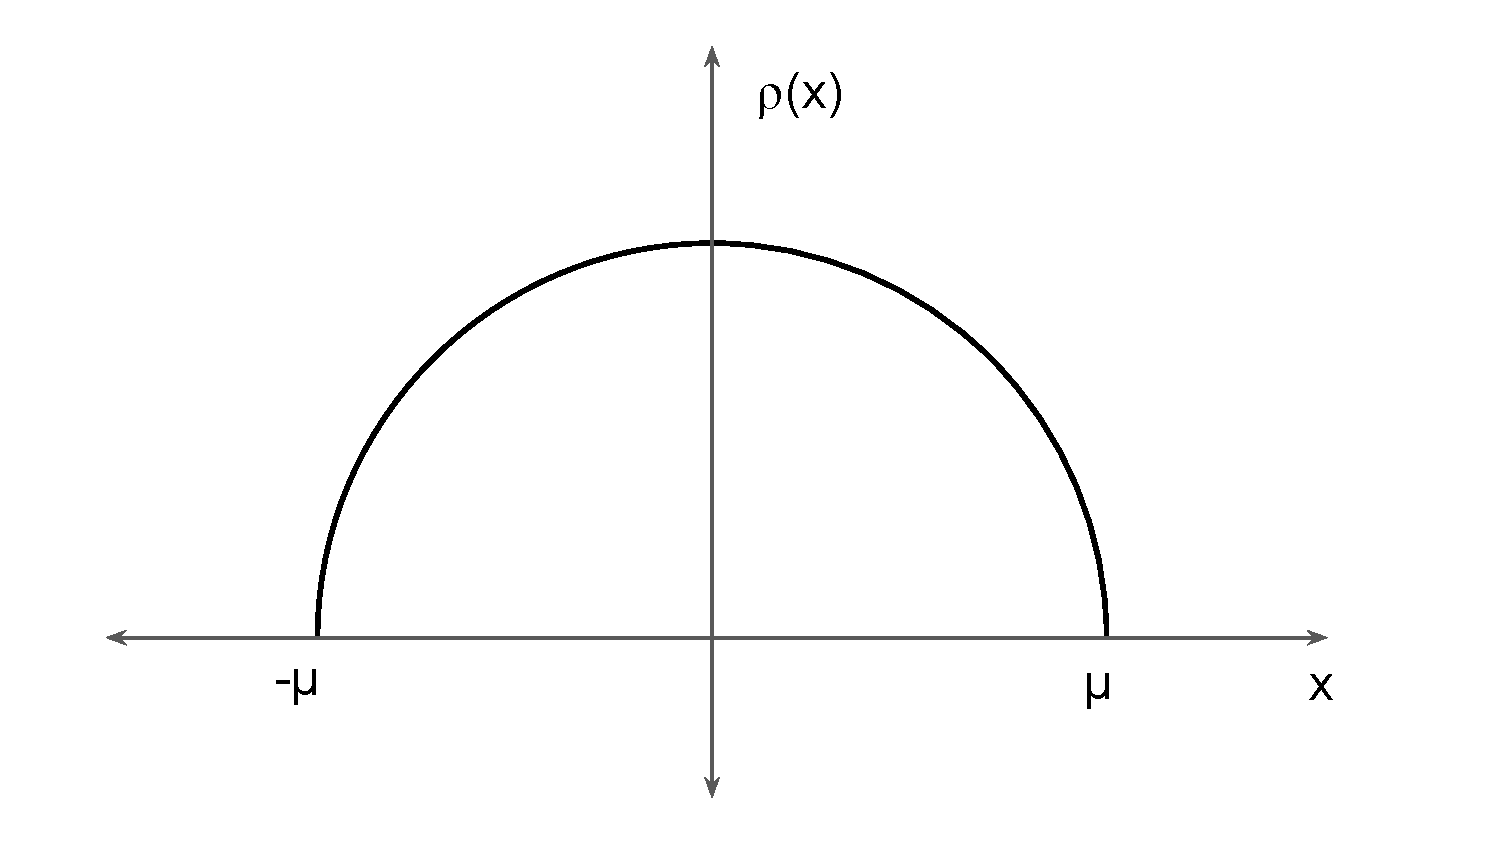
\includegraphics[width=0.8\textwidth]{Images/semicircle.pdf}}
 \caption{\label{fig:semicircle} Wigner's semicircle distribution, solution to the Gaussian unitary ensemble (GUE).}
\end{center}
\end{figure}

For the $\mathcal{N}=2^*$ SYM, the kernel is
\begin{equation}
 K(x)=\dfrac{1}{x}-\mathcal{K}(x)+\dfrac{1}{2}\,\mathcal{K}(x+MR)+\dfrac{1}{2}\,\mathcal{K}(x-MR),
\end{equation}
where 
\begin{equation}
 \mathcal{K}(x) \equiv -\dfrac{H'(x)}{H(x)} 
                = 2x\sum_{n=1}^{\infty} \left(\dfrac{1}{n}-\dfrac{n}{n^2+x^2} \right),
\end{equation}
and much more interesting features show up in the saddle-point solution, as shown in figure \ref{fig:phaseDiagram}.
Let us briefly review these results.


In the strong-coupling regime, the bulk of the distribution is also a semicircle but with a rescaled endpoint:
\begin{equation}\label{semicircleN=2*}
 \rho(x) = \dfrac{2}{\pi \mu^2} \sqrt{\mu^2-x^2}, 
 \quad
 \mu=\dfrac{\sqrt{\lambda (1+(MR)^2)}}{2\pi},
 \quad (\lambda \rightarrow \infty).
\end{equation}
This is due to the fact that the kernel is approximately a Hilbert kernel \cite{Buchel:2013id}:
\begin{equation} \label{Kapprox}
 K(x) \approx \dfrac{1+(MR)^2}{x}, \quad (\lambda \rightarrow \infty).
\end{equation}
Close to the edge-points, this approximation no longer holds,
and it was the goal of Paper I to find the endpoint distribution in the strong coupling regime.

We computed the endpoint distribution exactly using the so-called Wiener-Hopf method, 
which is essentially the Fourier transform of the convolution integral in \eqref{saddlepointEq} in a semi-infinite interval 
(zero being at the endpoint),
that relies on a certain factorization of the kernel.

The distribution exhibits oscillatory behavior with a period proportional to the scale $M R$. 
In the decompactification limit $MR\rightarrow \infty$ (but $\mu\gg MR$ because we remain in the strong coupling limit), 
the peaks of the oscillation diverge, see figure \ref{fig:phaseDiagram}.
The analytical endpoint distribution at strictly infinite coupling and flat space, with $\xi\equiv\mu-x$, is summarized below:
\begin{equation}
 \rho(\xi )= \frac{2^{3/2}}{\pi \mu^{3/2}}
% \frac{\sqrt{2 M R}}{\pi \mu^{3/2}}
 \begin{cases}
   MR \sqrt{\xi}, 
   &\quad (\xi \sim 1)\\
   \dfrac{\sqrt{M R}}{2}\sum_{k=0}^{\left[\frac{\xi }{MR}\right]}
             \left(\left\{\frac{\xi }{MR}\right\} + k\right)^{-1/2}
   &\quad (\xi \sim M R),
 \end{cases}
\end{equation}
where $[\cdot]$ and $\{\cdot\}$ denote the integer and the fractional part, respectively, 
and $\mu=MR\sqrt{\lambda}/(2\pi)$, from \eqref{semicircleN=2*}.

Physically, the cusps appear due to a resonance phenomena 
\begin{equation}
m_{ij} = |a_i-a_j \pm MR| \approx 0
\end{equation}
of very light states in the hypermultiplet sector.
Similar features were already observed for finite couplings in the flat space limit \cite{Russo:2013qaa},
and it was numerically shown that there are infinite-many critical couplings defined by 
\begin{equation}
 \mu = g(\lambda_c^{(n)}) M R, \quad g(\lambda_c^{(n)}) = \dfrac{n}{2}, \quad n=1,\ldots
\end{equation}
This means there are infinitely many phase transitions, where the phases are distinguished by the number of cusps of the distribution,
and the coupling $\lambda$ is the order parameter.
At strong coupling, the critical behavior persists and matches with the one obtained from the decompactification limit, 
hence these two limits commute \cite{Zarembo:2014ooa}.




\begin{figure}[t]
\begin{center}
 \centerline{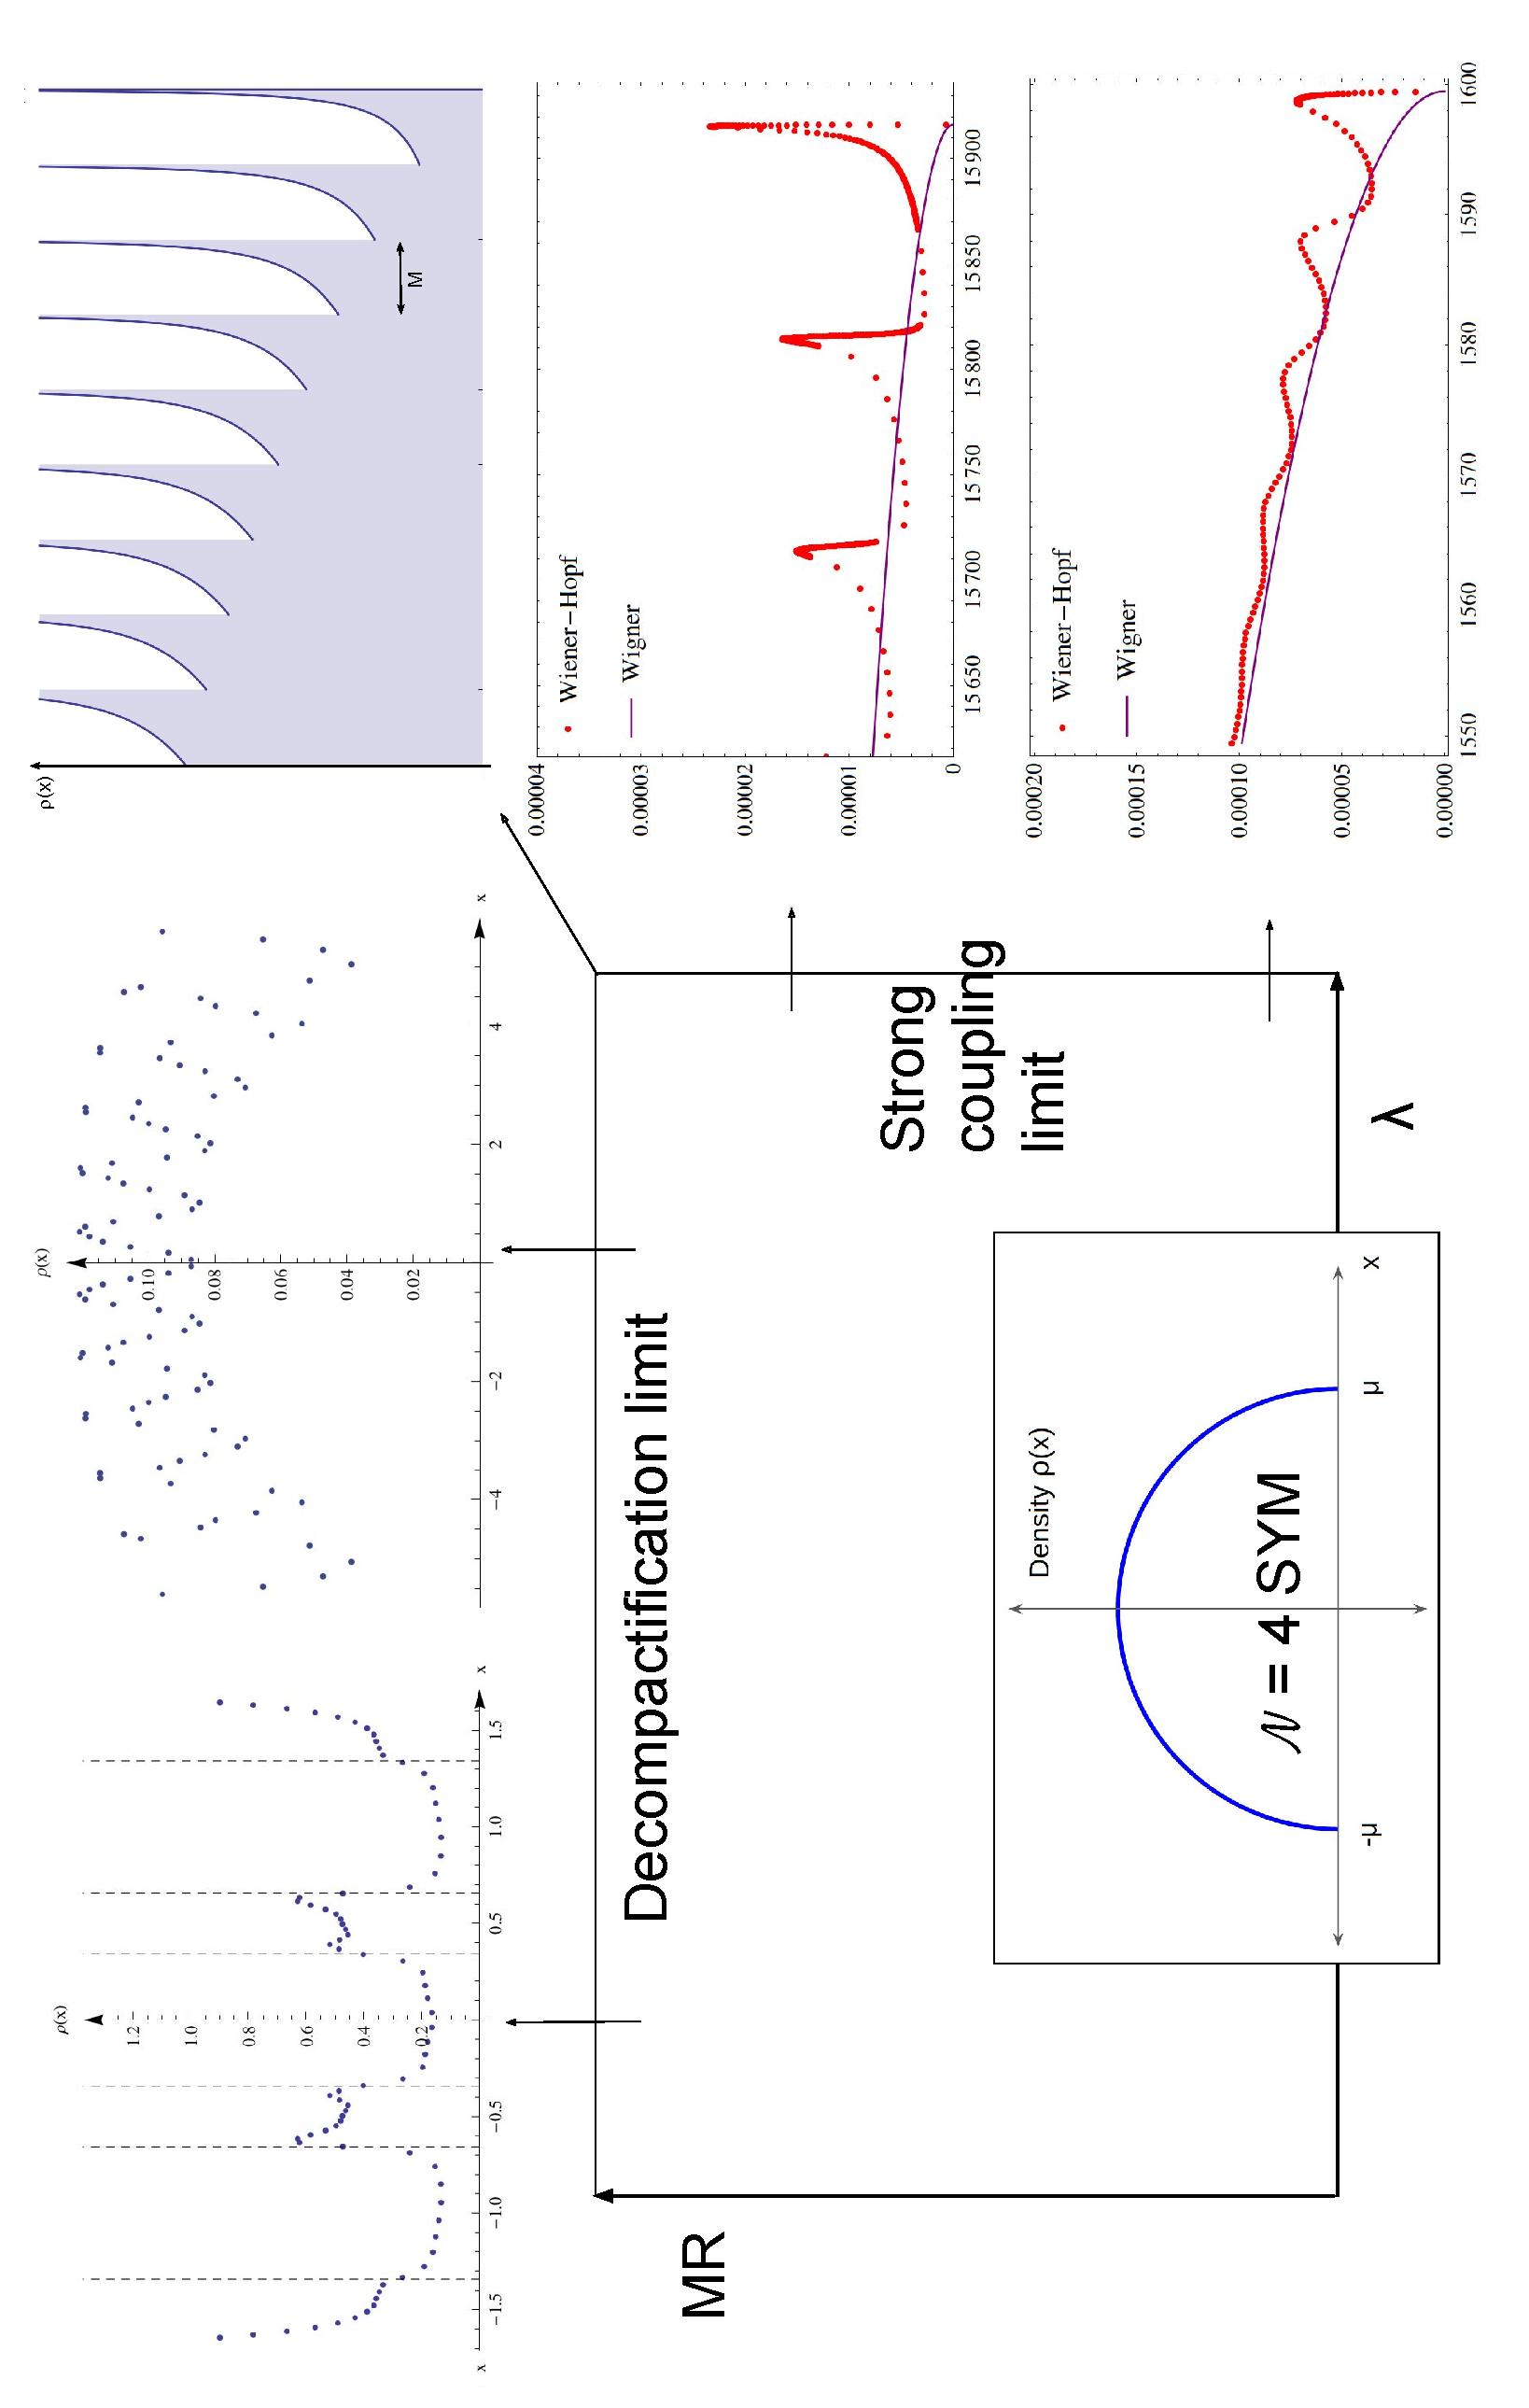
\includegraphics[width=0.9\textwidth]{Images/phaseDiagram.pdf}}
\end{center}
\caption{\label{fig:phaseDiagram} Phase diagram for the partition function of $\mathcal{N}=2^*$ SYM on $S^4$, in the large $N$ limit. 
The plots at the decompactification limit are taken from \cite{Russo:2013qaa}, and the ones at strong coupling limit are from Paper I, where only close to the endpoint is shown and $R=1$.
In the zero mass limit, we have $\mathcal{N}=4$ SYM, where the distribution is the Wigner semicircle for any coupling.}
\end{figure}


Such phase transitions are common among large-$N$ matrix models, 
and have been observed in e.g. ABJM models \cite{Anderson:2014hxa}, 5d $\mathcal{N}=1$ SYM with massive matter multiplets \cite{Nedelin:2015mta}.
In our case, the gauge/string duality in principle gives us an opportunity to understand them from the point of view of gravity.
The physical observables we use to probe the infinite-coupling phase are Wilson loops, the topic of the next chapter.








% \section{Action }

% Let us first review how to obtain the actions of our theories. 
% We will start with the action of $\mathcal{N}=4$ SYM on $\mathbb{R}^{3,1}$. 
% It is convenient to use the language of $\mathcal{N}=1$ SYM in $\mathbb{R}^{9,1}$, 
% from which all supersymmetric actions for lower dimensional Yang-Mills theory can be obtained from (cite someone).
% 
% The action is 
% \begin{equation}
%  S = \int d^4 x\, \sqrt{g} \mathcal{L}.
% \end{equation}
% 
% The Lagrangian density for $\mathcal{N}=4$ SYM on $S^4$:
% \begin{equation}
%  \mathcal{L}_{$\mathcal{N}=4$} = -\dfrac{1}{g_{YM}^2} 
%     \text{tr}\left(
%       \frac{1}{2}F_{MN}F^{MN} - \Psi \Gamma^M D_M \Psi  + \dfrac{2}{r^2} \Phi_A \Phi^A
%     \right).  
% \end{equation}
% For $\mathcal{N}=2^*$ SYM, we add mass to the hypermultiplet (in the covariant derivatives),
% \begin{equation}
%  \mathcal{L}_{$\mathcal{N}=2$^*} = 
% 		     -\dfrac{1}{g_{YM}^2} 
% 			   \text{tr} \left(
% 			      \frac{1}{2}F_{MN}F^{MN} - \Psi \Gamma^M D_M \Psi  + \dfrac{2}{r^2} \Phi_A \Phi^A
% 			      -\dfrac{1}{4 r} R_{ki} M_{kj} \Phi^i \Phi^j - K_i K^i
% 			    \right). 
% \end{equation}
% where the last term is added in order to have an off-shell susy so that the localization can be applied.